\documentclass[12pt]{article}
\usepackage{graphicx}
\usepackage{epstopdf}
\usepackage{enumerate}
\begin{document}

\section*{Exercise 1}

\subsection*{Question 1}
The rate at which the packets are received at node 1 converges to a constant value of around 500kbytes/s which equals the maximum download speed of 4Mbit/s. The little hills on top of the download rate can be explained by the inaccuracy of the perl visualization script.
\begin{figure}[h]
\centerline{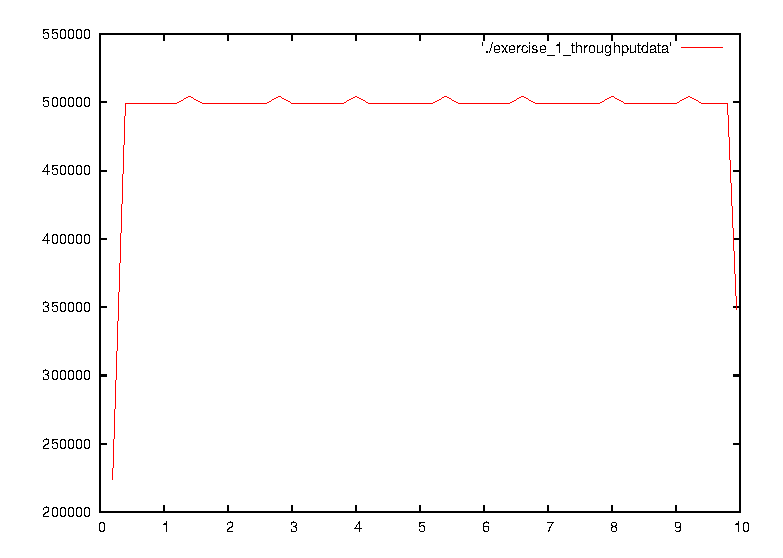
\includegraphics{pictures/E1Q1.eps}}
\caption{Caption 1}
\label{fig:question1}
\end{figure}

\subsection*{Question 2}
In the beginning of the TCP transfer the slow start is observed. When the UDP transmission kicks in, a significant drop in TCP throughput is observed. This is caused by the upload bandwidth limitation of the cable modem: TCP sends an acknowledgement for each received packet but the upload line is congested with UDP traffic as can be seen on the figure above. TCP throughput drops because acknowledgements are lost due to the overloaded buffer. After the loss of these acknowledgements the slow start mechanism of TCP will kick in again.
\begin{figure}[h]
\centerline{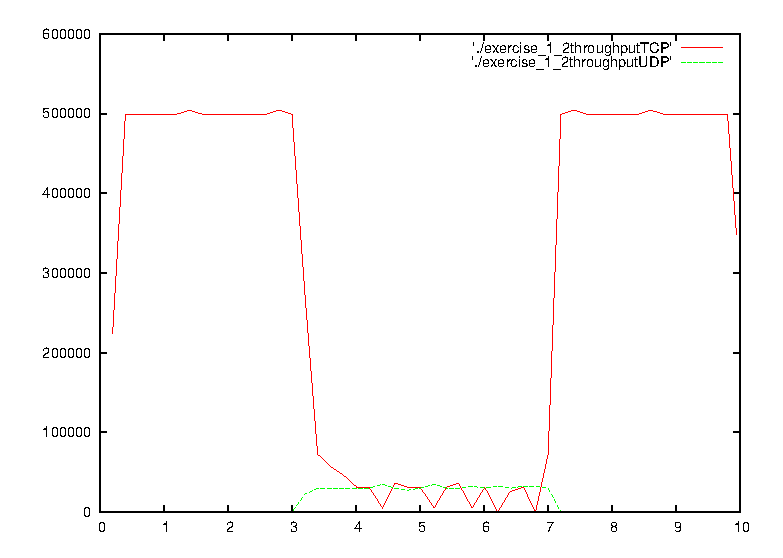
\includegraphics{pictures/E1Q2.eps}}
\caption{Caption 2}
\label{fig:question2}
\end{figure}

\subsection*{Question 3}
the acknowledgements of the TCP connection can then be transferred. If the assigned bandwidth for TCP is large enough to transfer the acknowledgements without congesting the buffer, the TCP throughput will sustain its maximum value. The UDP throughput will adapt to the assigned bandwidth.  

\subsection*{Question 4}
If we take the case where the 100 Mbit uplinks and downlinks are preserved, the traffic will be even more distorted. Because a bigger packet loss rate occurs at the buffers even more TCP acknowledgements will be discarded which results in a lower TCP throughput. UDP throughput also drops 

\subsection*{Question 5}
The TCP throughput doesn't drop that much as the situation where the rate of sending UDP packets isn't limited to 30kbytes/s. Although TCP experiences some jitter as it needs a higher bandwidth to transmit all its acknowledgements immediately. A possible solution to this jitter would be to increase TCP packet size and by this reduce the acknowledgement rate which leads to a maximum use of the 4 Mbit bandwidth.
\begin{figure}[h]
\centerline{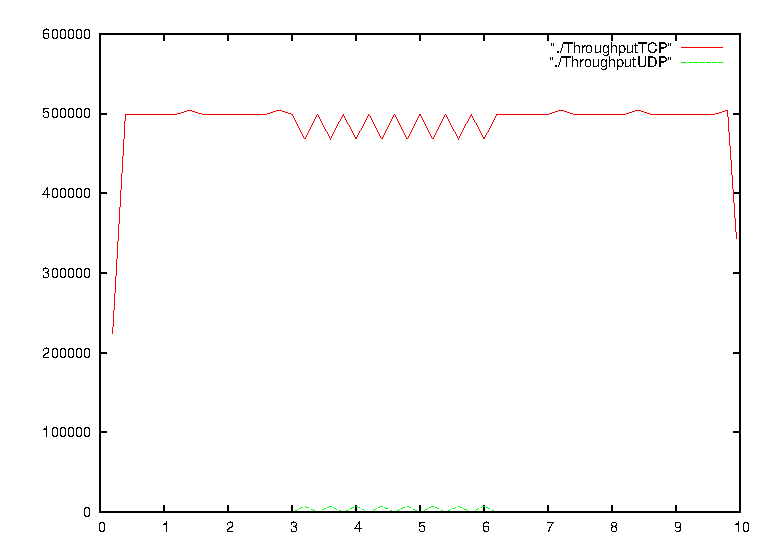
\includegraphics{pictures/E1Q5.eps}}
\caption{Caption 5}
\label{fig:question5}
\end{figure}

\subsection*{Question 6}
\begin{enumerate}[a)]
\item
With 10 users the amount of users and bandwidth scale with the same factor, so the performance will be the same.
When there are only 5 users using the network, one can reach a better performance If the UDP traffic also increases by the same factor; the TCP traffic will have twice as much bandwidth available.
\item
Yes, the performance will be more oscillating because the available bandwidth on the network varies randomly. Other users will suffer when one user decides to have a lot of UDP traffic because this UDP traffic obstructs acknowledgements from the TCP traffic which results in time-outs and thereby congestion.
\end{enumerate}

\section*{Exercise 1}

\subsection*{Question 1}
From the graph we can see that when the web traffic bursts start at 5.0 s, the long lasting ftp application does not immediately experience a drop in throughput. This is due to the slow start mechanism of the TCP connection which only reaches the maximum throughput at around 6.0s. The burst of HTTP requests will cause congestion which results in retransmission of dropped packets. We can see this on the graph where the burst traffic lasts until 8.0 s instead of 7.0 s. The bursts of HTTP traffic beginning on 10.0 s and 15.0 s can be analyzed analogously.
\begin{figure}[h]
\centerline{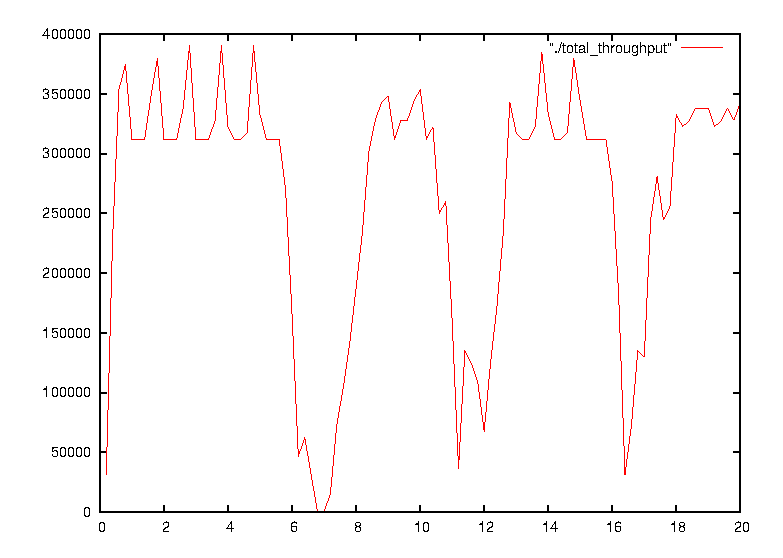
\includegraphics{pictures/E2Q1.eps}}
\caption{Caption E2Q1}
\label{ex2:question1}
\end{figure}

\subsection*{Question 2}
The different phases of the TCP algorithm are the slow start phase and the congestion avoidance phase in which the window size grows exponentially and linearly respectively. We can see this on the graph: The algorithm begins in the slow start phase and when the window size equals the slow start threshold it continues nearly linearly in the congestion avoidance phase. When congestion occurs and is detected, the window size will drop and the algorithm will start over again. A new threshold will also be calculated when congestion occurs. The value of this threshold is equal to half the value of the current slow start threshold.
\begin{figure}[h]
\centerline{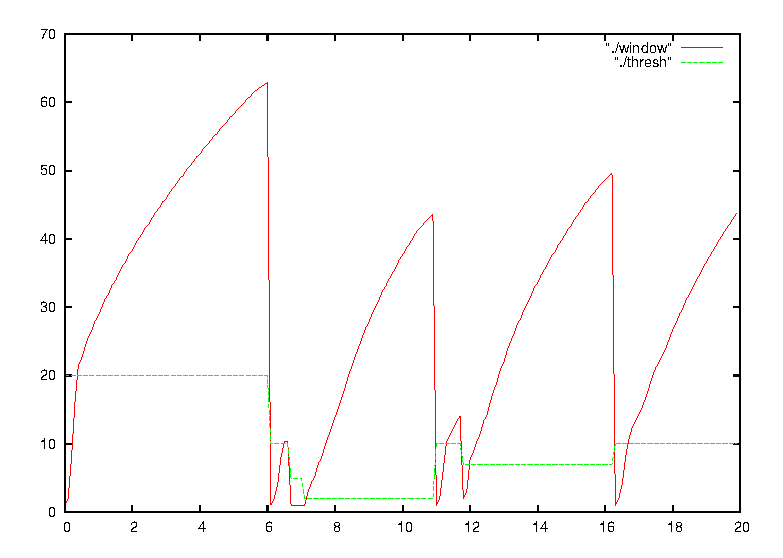
\includegraphics{pictures/E2Q2.eps}}
\caption{Caption E2Q2}
\label{ex2:question2}
\end{figure}

\subsection*{Question 3}
The additive increase/multiple decrease (AIMD) algorithm is used in TCP to make a feedback loop based on congestion signals. As congestion is a bad thing to happen because it also influences other clients on the network, a rapid decrease in traffic is needed to minimize the effect of the congestion. This is done by multiple decrease whereas when the network is not congested one can slowly increase the traffic with additive increase. It is shown by Chiu et al.1 that this asymmetry in buildup and break down speeds results in convergence to an optimal point.

The first interval where the TCP congestion avoidance algorithm is active is [0.45 – 5.45] as can be seen on the graph.

\subsection*{Question 4}
The difference between Tahoe and Reno lies in the fact that when congestion occurs, Tahoe always reduces the window size to 1 whereas Reno will perform fast recovery. This fast recovery will 
ensure that after 3 received duplicate acknowledgements the packet has not been transmitted succesfully. The congestion window size will be halved instead of lowered to 1 as with Tahoe.When time-outs occur, Reno acts the same way as Tahoe: the congestion window size will drop to 1 MSS.
\begin{figure}[h]
\centerline{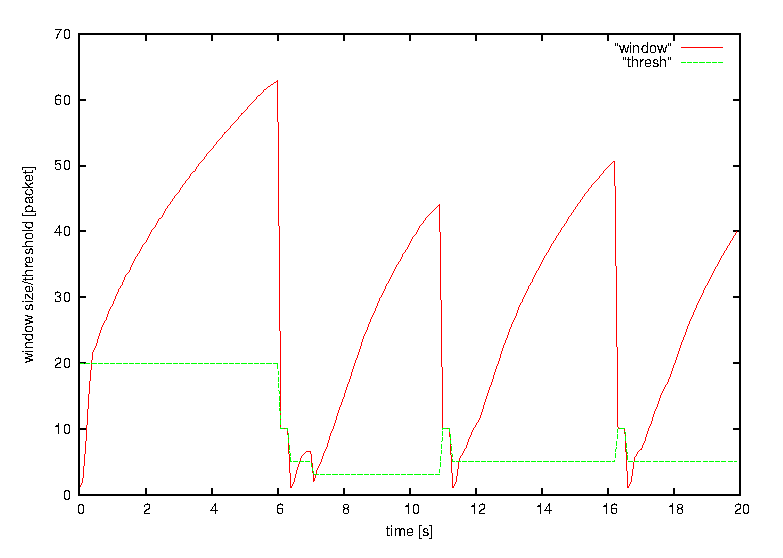
\includegraphics{pictures/E2Q4.eps}}
\caption{Caption E2Q4}
\label{ex2:question4}
\end{figure}

\end{document}
